\documentclass[11pt]{article}

\usepackage[margin=1in]{geometry}
\usepackage{booktabs}
\usepackage{graphicx}
\usepackage{amsmath}
\usepackage{amssymb}
\usepackage{hyperref}
\usepackage{xcolor}

\hypersetup{colorlinks=true, linkcolor=blue, urlcolor=blue}

\newcommand{\sep}{\texttt{x}}
\newcommand{\subj}[1]{\texttt{a\_#1}}
\newcommand{\obj}[1]{\texttt{b\_#1}}
\newcommand{\rel}[1]{\texttt{r\_#1}}
\newcommand{\fatt}[1]{\texttt{f\_#1}}
\newcommand{\gatt}[1]{\texttt{g\_#1}}
\newcommand{\Rsem}{R_{\mathrm{sem}}}
\newcommand{\Rrnd}{R_{\mathrm{rnd}}}

\title{Linear vs.\ Nonlinear Storage of Two Synthetic Relations\\ at Exactly Matched Frequency}
\author{factual-recall-mechanisms}
\date{2026-07-03}

\begin{document}
\maketitle

\section{Question and result in one paragraph}

One small transformer is trained for \textbf{exactly one epoch} on a synthetic corpus containing two relations with \emph{identical frequency statistics at every level} (same subjects, same 32 candidate objects, same number of triples, same number of occurrences per triple). The relations differ only in their semantics: $\Rsem$ maps each subject to the object determined by one of the subject's hidden attributes; $\Rrnd$ maps each subject to a random object. A single analysis metric is used: an affine map fitted by ordinary least-squares linear regression from subject representations to object representations, evaluated on held-out subjects. At 64 occurrences per triple both relations are recalled perfectly on their training triples, i.e.\ both are fully learned; yet the regression identifies the correct object for held-out subjects with accuracy $0.89 \pm 0.06$ for $\Rsem$ and $0.02 \pm 0.02$ ($=$ chance) for $\Rrnd$, replicated over three seeds. The semantic relation is stored in a linearly decodable, generalizing format; the random relation is memorized non-linearly. Raising the frequency of $\Rrnd$ facts from 1 to 64 occurrences never makes it linear, and the linear format of $\Rsem$ is already in place when every triple has occurred only once.

\section{Data}

\paragraph{Vocabulary (265 tokens).}
A separator \sep; two relation tokens \rel{0}, \rel{1}; 192 subject tokens $\subj{0},\dots,\subj{191}$; 32 object tokens $\obj{0},\dots,\obj{31}$; 32 attribute tokens $\fatt{0},\dots,\fatt{31}$; 6 attribute tokens $\gatt{0},\dots,\gatt{5}$.

\paragraph{Entities and attributes.}
Subject $\subj{i}$ carries the attribute pair $(f_{i \bmod 32},\ g_{\lfloor i/32\rfloor})$, so the 192 subjects realize each of the $32 \times 6$ attribute combinations exactly once. Object $\obj{j}$ carries $(f_{(j+3) \bmod 32},\ g_0)$.

\paragraph{Sentences.}
All training sentences have five tokens:
\begin{center}
\begin{tabular}{ll}
attribute sentence & \sep\ $\subj{i}$\ \fatt{p}\ \gatt{q}\ \sep \quad and \quad \sep\ $\obj{j}$\ \fatt{p}\ \gatt{q}\ \sep\\
relation triple & \sep\ $\subj{i}$\ $\rel{r}$\ $\obj{t}$\ \sep
\end{tabular}
\end{center}

\paragraph{Relations.}
\[
\Rsem(a_i) = b_{f(i)}, \qquad \Rrnd(a_i) = b_{\rho(i)},
\]
where $f(i) = i \bmod 32$ is the subject's own $f$-attribute index --- so the semantic target is the object whose $f$-attribute is the subject's, shifted by 3 --- and $\rho$ is a seed-dependent balanced random assignment onto the same 32 objects, independent of the attributes.
Concrete example (seed 19): \subj{37} has attributes $(\fatt{5}, \gatt{1})$, so $\Rsem(\subj{37})=\obj{5}$ (whose attribute sentence reads \sep\ \obj{5}\ \fatt{8}\ \gatt{0}\ \sep), while $\Rrnd(\subj{37})=\obj{27}$. The corresponding training sentences are \sep\ \subj{37}\ \rel{0}\ \obj{5}\ \sep\ and \sep\ \subj{37}\ \rel{1}\ \obj{27}\ \sep.

\paragraph{Split and exact frequency matching.}
For every \fatt-value, 4 of its 6 subjects are \emph{trained} and 2 are \emph{held out} (128 trained, 64 held-out subjects; seed-dependent). $\rho$ is constructed balanced within both groups. Consequently, under \emph{both} relations: every trained subject occurs in exactly one triple per relation; every object is the target of exactly 4 trained and 2 held-out subjects; both relations contribute exactly 128 training triples, each repeated the same number of times ($F$). The two relations are therefore indistinguishable by any frequency statistic; only the assignment semantics differ. Held-out subjects appear in attribute sentences but never in any relation triple. These invariants are asserted by \texttt{tests/test\_linear\_shift.py}.

\section{Model and training}

\begin{center}
\begin{tabular}{ll}
\toprule
Model & causal transformer, 1 layer, hidden 64, 4 heads, context 8\\
Embeddings & input and output embeddings untied; all weights $\mathcal{N}(0, 0.02^2)$\\
 & \textbf{no} attribute-based initialization; nothing frozen; no loss reweighting\\
Parameters & 84{,}288\\
Corpus & every attribute sentence $\times A{=}128$ ($= 28{,}672$ sentences)\\
 & $+$ 128 triples per relation, each $\times F$ ($F \in \{1,4,16,64\}$)\\
Training & \textbf{exactly one epoch}: a single pass over the shuffled corpus\\
Steps & 452 ($F{=}1$) to 704 ($F{=}64$) steps at batch size 64\\
Objective & untweighted next-token cross-entropy on all positions\\
Optimizer & AdamW, constant LR $10^{-3}$ after 5 linear warmup steps,\\
 & weight decay 0, gradient clip 1.0\\
Seeds & 19, 31, 47 (control data assignment, initialization, and data order)\\
\bottomrule
\end{tabular}
\end{center}

At $F{=}1$ every relation triple occurs exactly once in the entire training history of the model.

\section{The metric}

A single analysis metric is used, as an operationalization of ``the relation is an affine transformation'':

\begin{quote}
Fit $\hat W, \hat b$ by ordinary least-squares linear regression from the subject's \emph{input embedding} $s_i \in \mathbb{R}^{64}$ to the target object's \emph{output embedding} (unembedding row) $o_{R(i)} \in \mathbb{R}^{64}$, using the 128 trained pairs. For each of the 64 held-out subjects, predict $\hat W s_j + \hat b$ and select the nearest object row by cosine similarity among all 32 objects. Report the fraction of held-out subjects for which the selected object is $R(j)$. Chance is $1/32 \approx 0.03$.
\end{quote}

This replaces all top-$k$ and accuracy-style analysis metrics of earlier drafts. The identification step avoids the earlier ambiguity objection: for every subject, exactly one object is correct under each relation. In addition, one \emph{learning check} (not an analysis metric) is recorded: greedy next-token recall of the model on prompts \sep\ $\subj{i}$\ $\rel{r}$, for trained and held-out subjects, which verifies whether the facts were learned at all.

\section{Results}

\begin{table}[h]
\centering
\begin{tabular}{rcccccc}
\toprule
 & \multicolumn{2}{c}{probe accuracy (held-out)} & \multicolumn{2}{c}{recall (trained)} & \multicolumn{2}{c}{recall (held-out)}\\
$F$ & $\Rsem$ & $\Rrnd$ & $\Rsem$ & $\Rrnd$ & $\Rsem$ & $\Rrnd$\\
\midrule
1  & $1.000 \pm .000$ & $.031 \pm .013$ & .029 & .010 & .016 & .010\\
4  & $1.000 \pm .000$ & $.016 \pm .013$ & .055 & .034 & .057 & .031\\
16 & $0.990 \pm .007$ & $.036 \pm .007$ & .672 & .167 & .635 & .031\\
64 & $0.891 \pm .056$ & $.016 \pm .022$ & \textbf{1.000} & \textbf{1.000} & .995 & .031\\
\midrule
control: no triples & $1.000 \pm .000$ & $.021 \pm .015$ & -- & -- & .000 & .000\\
\bottomrule
\end{tabular}
\caption{Mean $\pm$ sd over seeds 19/31/47, at $A{=}128$ attribute-sentence occurrences. $F$ is the number of occurrences of each of the 128 triples per relation. Recall columns are the learning check.}
\label{tab:main}
\end{table}

\begin{figure}[h]
\centering
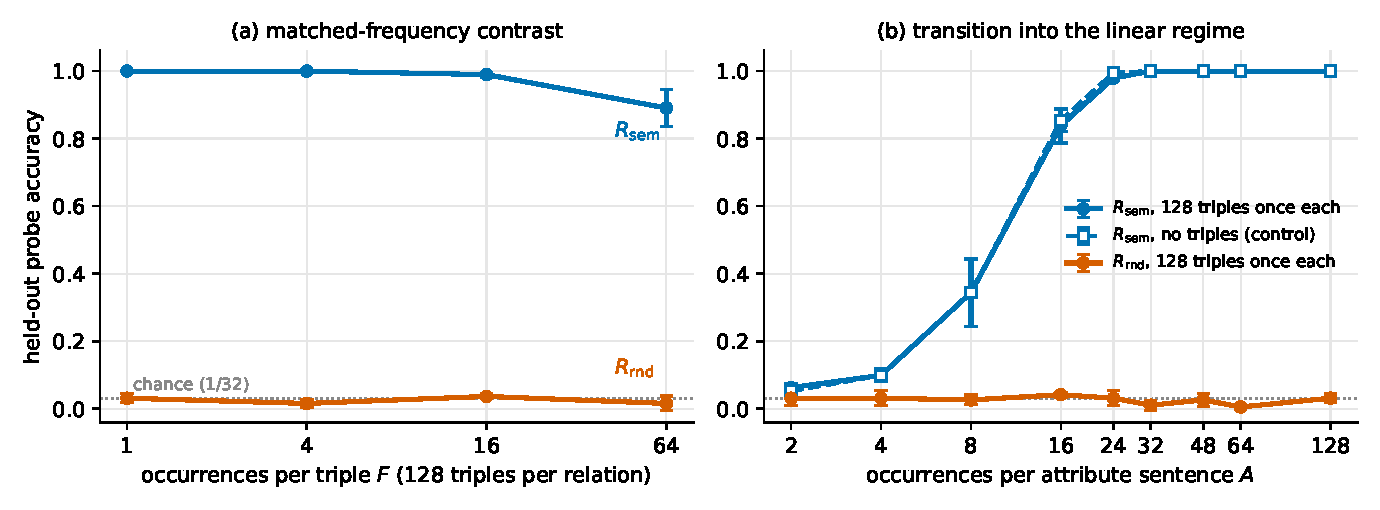
\includegraphics[width=\textwidth]{figures/linear_shift_results.pdf}
\caption{(a) Held-out probe accuracy vs.\ occurrences per triple: $\Rsem$ is linear at every frequency (slightly degrading at $F{=}64$), $\Rrnd$ is never linear. (b) Probe accuracy at $F{=}1$ as a function of attribute-sentence occurrences $A$: the transition into the linear regime is sharp, and identical with 128 once-occurring triples (solid) and with no triples at all (dashed control).}
\label{fig:results}
\end{figure}

\paragraph{Finding 1: with matched frequency, semantics decides the format (Table~\ref{tab:main}, $F{=}64$).}
Both relations reach perfect recall of all 128 training triples --- both are fully learned by the model, from data with identical frequency statistics. The affine probe transfers to held-out subjects almost perfectly for $\Rsem$ ($0.891 \pm 0.056$; and the model itself generalizes behaviorally, held-out recall $0.995$) and is at chance for $\Rrnd$ ($0.016 \pm 0.022$; held-out recall at chance). The random relation is thus stored, but stored \emph{non-linearly}: no affine map over the same representations accounts for it.

\paragraph{Finding 2: single occurrences already put the semantic relation in the linear regime.}
At $F{=}1$ --- every triple exactly once, in a single epoch --- the probe is already at $1.000$ for $\Rsem$ and at chance for $\Rrnd$. Increasing frequency does not create the linear format (Fig.~\ref{fig:results}a, $\Rrnd$ flat at chance) and if anything slightly erodes it for $\Rsem$ ($1.000 \rightarrow 0.891$), consistent with high-frequency memorization competing with the linear solution.

\paragraph{Finding 3: the nonlinear$\rightarrow$linear transition is driven by attribute knowledge, not by triple repetition.}
Sweeping the number of occurrences $A$ of each attribute sentence at $F{=}1$ (Fig.~\ref{fig:results}b) produces a sharp transition of the $\Rsem$ probe from chance to ceiling ($0.05 \rightarrow 0.10 \rightarrow 0.34 \rightarrow 0.85 \rightarrow 1.00$ for $A = 2,4,8,16,24$). The control with \emph{zero} relation triples produces the same curve. Hence the affine subject$\to$object map is carried by the attribute geometry that the model builds from attribute sentences; the once-seen $\Rsem$ triples are consistent with that geometry (and at higher $F$ the relation visibly uses it: held-out behavioral recall $0.995$), whereas $\Rrnd$ triples cannot be, at any frequency.

\section{What this does and does not show}

\begin{itemize}
  \item \textbf{Shown:} two relations with exactly matched frequency statistics but different semantics end up in different storage formats --- affine/generalizing vs.\ memorized/non-affine (Finding 1); a relation whose facts each occur \emph{once} can already sit in the linear regime, and frequency is not what creates linearity (Finding 2); the transition into the linear regime is sharp, but its driver is the amount of attribute (scaffold) training (Finding 3).
  \item \textbf{Not shown:} that the relation triples themselves \emph{cause} the nonlinear$\rightarrow$linear transition when each fact occurs only once. The $A$-sweep control (Fig.~\ref{fig:results}b, dashed) demonstrates the opposite in this setting. We attempted three designs in which the probe could only succeed through triple-driven structure (a one-to-one relation requiring per-fact output rows; a relation defined by the conjunction of two attributes, up to $49{,}152$ distinct facts; both with hidden-state probes): under the strict single-occurrence, one-epoch regime none produced above-chance probe transfer, because each fact contributes exactly one gradient and per-fact structure cannot form. Also note that at $F{=}1$ the model does not yet reproduce individual triples behaviorally (recall $\approx .03$); the $F{=}1$ statement is about the representational format, not about recall.
  \item \textbf{Superseded:} the ``single-exposure phase shift'' reported in earlier drafts of this document (probe rising $0.27 \rightarrow 0.95$ during a single-exposure phase) is an artifact and should not be cited: its regression was fitted on a growing set of pairs (10 at the first snapshot, $>$500 later) over embeddings that had been \emph{initialized} from the attribute geometry. With a fixed-size probe and standard initialization the effect disappears. All earlier experiments using \texttt{structured\_embedding\_init}, targeted-row updates, pilot-triple repetition, or top-$k$ metrics are superseded by the present setup.
\end{itemize}

\section{Reproduction}

Implementation: \texttt{experiments/factual\_recall/linear\_shift.py} (self-contained: world, corpus, training, probe; $\sim$450 lines). Design invariants: \texttt{experiments/tests/test\_linear\_shift.py}. From \texttt{experiments/}:

\begin{small}
\begin{verbatim}
# Table 1 / Figure (a): one seed per command (19, 31, 47), ~1 min each on one GPU
uv run python -m factual_recall.linear_shift --world category --probe embedding \
  --seeds 19 --k-values 0,128 --occurrences 1,4,16,64 --attr-repeats 128 \
  --device cuda --output-dir factual_recall/results/final_category_seed19

# Figure (b): attribute-exposure sweep at F=1, per seed and A
uv run python -m factual_recall.linear_shift --world category --probe embedding \
  --seeds 19 --k-values 0,128 --occurrences 1 --attr-repeats 8 \
  --device cuda --output-dir factual_recall/results/final_category_arsweep_seed19_ar8
# ... repeated for A in {2,4,8,16,24,32,48,64,128}

# Aggregation and figure
# factual_recall/results/final_summary/summary.json, make_figure.py

# Design invariants
uv run pytest tests/test_linear_shift.py -q
\end{verbatim}
\end{small}

Raw per-run metrics (including probe $R^2$/cosine and losses, recorded but not reported) are in \texttt{factual\_recall/results/final\_category\_*/linear\_shift\_metrics.json}.

\end{document}
